\documentclass[12pt, titlepage]{article}

\usepackage{booktabs}
\usepackage{enumerate}
\usepackage{graphicx}
\usepackage{mdwlist}
\usepackage{tabularx}
\usepackage{float}
\usepackage{hyperref}
\usepackage{ulem}
\usepackage{xcolor}
\hypersetup{
    colorlinks,
    citecolor=black,
    filecolor=black,
    linkcolor=red,
    urlcolor=blue
}
\usepackage[round]{natbib}

\title{SE 3XA3: Software Requirements Specification\\super-refactored-mario-python}

\author{Team 203, Abstract Connoiseurs
		\\ Alexander Samaha, samahaa
		\\ Daniel Noorduyn, noorduyd
		\\ David Jandric, jandricd
}

\date{\today}

%\input{../Comments}%

\begin{document}

\maketitle

\pagenumbering{roman}
\tableofcontents
\listoftables
\listoffigures

\begin{table}[bp]
\caption{\bf Revision History}
\begin{tabularx}{\textwidth}{p{3cm}p{2cm}X}
\toprule {\bf Date} & {\bf Version} & {\bf Notes}\\
\midrule
Feb 4 2020 & 1.0 & Initial changes to the document \\
\textcolor{red}{April 6, 2020} & \textcolor{red}{1.1} & \textcolor{red}{Rev 1 Touch-ups}\\
\bottomrule
\end{tabularx}
\end{table}

\newpage

\pagenumbering{arabic}

This document describes the requirements for super-refactored-mario-python,
which is an implementation of the Super Mario Bros. game in Python. The template
for the Software Requirements Specification (SRS) is a subset of the
\href{RobertsonAndRobertson2012}{\textcolor{red}{Volere template}}. This
document serves to inform users and stakeholders of the overview of the project
including constraints and objectives this project hopes to meet.

\section{Project Drivers}

\subsection{The Purpose of the Project}
    The purpose of super-refactored-mario-python is to re implement and modify the age old Super Mario Bros. game in an open source environment. The team will finish the work started and left uncompleted, then look to add features \sout{that diverge from the original game} \textcolor{red}{that round of the base functionality of the original game}. The end result is a version of Super Mario Bros. that can be enjoyed by anyone with access to a computer with the proper libraries installed.

\subsection{\textcolor{red}{The Scope of the Project}}
    \textcolor{red}{The final version of Super Refactored Mario Bros will be a replica of the original Super Mario Bros game at its base functionality. It will be created using python3 and the corresponding libraries scipy and pygame. The special features such as multiple power-ups and moving pipes, flying enemies, etc. will not be implemented due to time constraints. Therefore the goal will be to organize and/or rewrite the existing code to create a base functionality replica.}

\subsection{The Stakeholders}

\subsubsection{The Client}
    The client for super-refactored-mario-python is the instructor and teaching assistants of the SFWRENG 3XA3 course.
\subsubsection{The Customers}
    The customers of this project are all with an interest in the original Super Mario Bros. game and open-source game development in general. This project will be available for anyone to download if they have access to a computer that satisfies the hardware and software requirements.
\subsubsection{Other Stakeholders}
    The original project owner has a vested interest in the completion of their unfinished project. This may include the integration of the changes and features put forward during the development cycle. Furthermore, the open-source Pygame community will have a vested interest in the propagation of its use to make video games. Finally, the development team also has a vested interest in the success of the project.
\subsection{Mandated Constraints}
    \textbf{Description:} The project shall use the Pygame library for Python game development.\\
    \textbf{Rationale:} The project is originally written with the Pygame library and will make it easier to continue using it.\\
    \textbf{Fit Criterion:} Running the game files with Python includes and runs the Pygame library.\\\\
    \textbf{Description:} The project shall follow the structure of deliverables outlined in the project schedule.\\
    \textbf{Rationale:} The project needs to follow a logical schedule to ensure completion of the product within the allotted time.\\
    \textbf{Fit Criterion:} The project is completed and all deliverables submitted by April 6th 2020.\\\\
    \textbf{Description:} The project shall use the Pygame library for Python game development.\\
    \textbf{Rationale:} The project is originally written with the Pygame library and will make it easier to continue using it.\\
    \textbf{Fit Criterion:} Running the game files with Python includes and runs the Pygame library.\\\\
\subsection{Naming Conventions and Terminology}
    \textbf{SFWRENG 3XA3} - The Software Engineering Practice and Experience: Software Project Management course instructed by Dr. Asghar Bokhari.\\
    \textbf{Super Mario Bros.} - The original arcade game released in 1985 for the Nintendo Entertainment System in North America.\\
    \textbf{Pygame} - Popular library for small open-source games written in Python.\\
    \textbf{Koopa} - Refers to a non-playable character in the Super Mario Bros. game that is encountered as an enemy. This character has a shell that can be used as a projectile.\\
    \textcolor{red}{\textbf{Koopa Shell} - The shell of the \textbf{Koopa} that can be used as a projectile.}\\
    \textbf{Regular enemy} - Refers to a non-playable character in the Super Mario Bros. game that is encountered as an enemy such as a Goomba.\\\
    \textcolor{red}{\textbf{Main Menu} - The initial menu where the user can determine what they want to do in the game.}\\
\subsection{Relevant Facts and Assumptions}
    \subsubsection{Facts}
    \begin{itemize}
        \item Pygame is a set of modules used to create video games written in Python. It encompasses graphics and sound libraries.
        \item The original repository contains 1390 lines of Python code.
    \end{itemize}
    \subsubsection{Assumptions}
    It is assumed that the user has access to a modern computer with the necessary Python interpreter installed along with the Pygame library and is able to run the files. Along with this, the user is expected to have working knowledge of running Python code from the command line. The user is assumed to have a keyboard and a mouse to be able to interact with the game. It is assumed that the user has installed all the required artefacts in a compatible operating system environment.

\section{Functional Requirements}

\subsection{The Scope of the Work and the Product}

\subsubsection{The Context of the Work}

\begin{figure}[H]
    \centering
    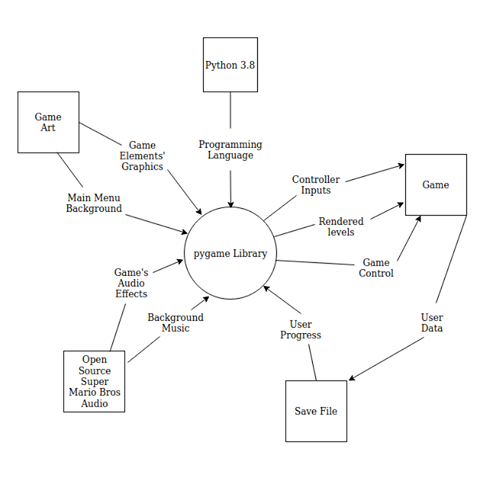
\includegraphics[width=\textwidth]{SRScontextdiagram.png}
    \caption{Game Context Diagram}
    \label{fig:contextdiagram}
\end{figure}

\subsubsection{Work Partitioning}

\begin{tabular}{|l|l|l|}
\hline
\textbf{Event} & \textbf{Input/Output} & \textbf{Summary} \\\hline
Player action  & \begin{tabular}{l}Player action(IN) \\ Change in game state(OUT)\end{tabular} &
\begin{tabular}{l}Respond to the users \\ input by updating the \\ game state accordingly. \end{tabular}  \\\hline

Collision & \begin{tabular}{l}Entity location(IN) \\ Change in game state(OUT)\end{tabular} &
\begin{tabular}{l} Update the game state \\ when there is \\ an entity collision.\end{tabular}\\\hline

\textcolor{red}{Save Game} & \begin{tabular}{l}\textcolor{red}{Finish Level(IN)} \\ \textcolor{red}{Change in High Score(OUT)}\end{tabular} &
\begin{tabular}{l} \textcolor{red}{Update the highscore} \\ \textcolor{red}{database for every} \\ \textcolor{red}{level completion.}\end{tabular}\\\hline
\end{tabular}

\subsubsection{Individual Product Use Cases}
The primary use case of this product is to be played from start to end, and get the best high-score. There will be a number of levels, and each will have a high score associated with it, for players to challenge themselves and constantly improve their score.
\textcolor{red}{Some specific use cases:}
\begin{enumerate}
  \item \textcolor{red}{'Main Menu': The user controls which option to select using the ARROW\_KEYS. The user is able to choose between entering levels, changing sound settings, and exiting the game.}
  \item \textcolor{red}{Controlling Mario: Once in a level, the user uses KEYBOARD\_LEFT, KEYBOARD\_RIGHT and KEYBOARD\_JUMP to control a player. Holding down KEYBOARD\_LEFT or KEYBOARD\_RIGHT moves Mario left or right until another entity blocks the way. Pressing KEYBOARD\_JUMP causes Mario to jump up.}
  \item \textcolor{red}{Pausing the Game: While midgame, the user can press KEYBOARD\_ESC to freeze gameplay. The user can then use ARROW\_KEYS to either return to the 'main menu' or continue playing.}
  \item \textcolor{red}{Beating a Level: When the user reaches the end of a level, the gameplay freezes and the user's score is compiled. The user is then transported to the beginning of the next level.}
  \item \textcolor{red}{Beating the Game: When the user reaches the end of the last level, having sequentially beat all previous levels, the user's score is compiled and the highscore is updated if the user's score is greater than the current highscore. Lastly, the user is transported to the 'main menu'.}
\end{enumerate}

\subsection{Functional Requirements}
\begin{enumerate}[{FR}1. ]
    \item When the user presses \sout{the 'W' key} \textcolor{red}{KEYBOARD\_JUMP}, the character shall jump.
    \item When the user \sout{presses the 'A' key} \textcolor{red}{holds down KEYBOARD\_LEFT}, the character shall move left.
    \item \sout{When the user presses the 'S' key, the character shall duck, making the characters size half of what it is.}
    \item When the user \sout{presses the 'D' key} \textcolor{red}{holds down KEYBOARD\_RIGHT}, the character shall move \sout{left} \textcolor{red}{right.}
    \item \sout{When the character is ducking, they shall be prevented from moving, until they stop ducking.}
    \item When the user jumps on top of a regular enemy, they shall die.
    \item When the user jumps on a 'Koopa', the 'Koopa' shall retract into its shell.
    \item If the user walks into, or jumps onto, the 'Koopa shell', it shall start sliding across the ground, and will bounce off walls and move in the opposite direction.
    \item If the player character \textcolor{red}{who doesn't have a power up} or enemy is hit by the shell, they shall die.
    \item If the player dies, they shall be reset to the beginning of the level and a life will be deducted.
    \item The player shall have 3 lives.
    \item If the player loses all 3 lives, they shall be returned to the main menu, and their high-score will be saved.
    \item When the player reaches \sout{a 'flagpole'} \textcolor{red}{the end of level}, they shall win the level, and be transported to the next.
    \item When the player finishes all levels in sequence, they shall \sout{be shown a 'You Win' screen, and} be transported to the main menu. Their high-score shall be saved.
    \item \textcolor{red}{When the user collides with the bottom of a power up box, a Mushroom will pop up out of the top and begin moving left and right resulting in it falling towards ground level.}
    \item \textcolor{red}{When the user collides with the mushroom power up, the mushroom will disappear and the user will changes from 'small Mario' to 'big Mario'.}
    \item \textcolor{red}{When the user is 'big Mario' and collides with an enemy, they shall be transformed back to 'small Mario' and have a period of invincibility.}
    \item \textcolor{red}{When the user collides with the underside of the random box, a coin will pop out of the top and revolve before dissappearing. The user's highscore will be updated accordingly.}
    \item \textcolor{red}{When the user collides with a floating coin in any level, the coin will disappear and the user's highscore will be updated accordingly.}
\end{enumerate}
\section{Non-functional Requirements}

\subsection{Look and Feel Requirements}
\begin{enumerate}[{LF}1. ]
    \item The product shall look extremely similar to the original Super Mario Bros.\\
    \textbf{Fit Criteria:} \sout{Users who are familiar with the original game} \textcolor{red}{TEST\_USERS} shall be able to navigate through the first level within \sout{1 minute and 30 seconds} \textcolor{red}{INITIAL\_NAV\_TIME}.
    \item The product shall have a modern looking menu.\\
    \textbf{Fit Criteria:} \sout{Users} \textcolor{red}{TEST\_USERS} shall be able to recognize all menu options within \sout{30 seconds} \textcolor{red}{INITIAL\_UNDERSTANDING\_TIME} of booting the game.
\end{enumerate}



\subsection{Usability and Humanity Requirements}

\subsubsection{Ease of Use Requirements}
\begin{enumerate}[{UH}1. ]
    \item The product shall be usable for anybody over the age of 10.\\
    \textbf{Fit Criteria:} Users shall be able to start a level within \sout{30 seconds} \textcolor{red}{UNDERSTAND\_TIME} of booting the game
    \item The product shall have simple, standard controls.\\
    \textbf{Fit Criteria:} Users shall move their character within \sout{10 seconds} \textcolor{red}{MOVEMENT\_TIME} of starting a level.
\suspend{enumerate}

\subsubsection{Personalization and Internationalization Requirements}
N/A

\subsubsection{Learning Requirements}
\resume{enumerate}[{[{UH}1.]}]
    \item The product shall be playable by a user after reading the in game tutorial.\\
    \textbf{Fit Criteria:} \sout{A test group of 20 users} \textcolor{red}{TEST\_USERS} shall read the tutorial and play the first level, $90$\% of the test group shall rate their experience as favourable regarding understanding game controls and rules.
    \item The product shall be playable by some users without reading the in game tutorial.\\
    \textbf{Fit Criteria:} \sout{A test group of 20 users} \textcolor{red}{TEST\_USERS} shall read the tutorial and play the first level, $50$\% of the test group shall rate their experience as favourable regarding understanding game controls and rules.
\suspend{enumerate}

\subsubsection{Understandability and Politeness Requirements}
\resume{enumerate}[{[{UH}1.]}]
    \item The product shall use simple language which can be understandable by $95$\% of users.\\
    \textbf{Fit Criteria:} A questionnaire will be authored and $95$\% of \sout{users} \textcolor{red}{TEST\_USERS} shall rate their experience positively in understanding the rules of the game.
    \item The product shall use standard icons indicative of their function to avoid confusion of the user.\\
    \textbf{Fit Criteria:} The game shall include all standard images of the original game.
    \item The product shall use a simple font which is easily read by all users.
    \textbf{Fit Criteria:} A questionnaire will be authored and $95$\% of \sout{users} \textcolor{red}{TEST\_USERS} shall rate their experience as favourable reading through the game menus.
\end{enumerate}

\subsubsection{Accessibility Requirements}
N/A



\subsection{Performance Requirements}

\subsubsection{Speed and Latency Requirements}
\begin{enumerate}[{PR}1. ]
    \item The product shall run at \sout{60 frames per second} \textcolor{red}{FRAME\_SPEED}.\\
    \textbf{Fit Criteria:} A play test shall be conducted \sout{with a group of 10 testers} \textcolor{red}{by TEST\_USERS} whose frame rates shall be captured through the first level of the game, the frame rate shall maintain \sout{60 frames per second} \textcolor{red}{FRAME\_SPEED} 95\% of the time under normal conditions.
    \item The product shall take no more than \sout{3 seconds} \textcolor{red}{the LOAD\_TIME} to load and display all resources.\\
    \textbf{Fit Criteria:} A play test shall be conducted \sout{with a group of 10 testers} \textcolor{red}{by TEST\_USERS} to confirm the game loads within \sout{3 seconds} \textcolor{red}{the LOAD\_TIME} 90\% of the time.
    \item The product shall not significantly slow down if there are \sout{100 entities} \textcolor{red}{TEST\_ENTITIES} displaying on the screen.\\
    \textbf{Fit Criteria:} A \sout{playtest} \textcolor{red}{play test} shall be conducted \sout{with a group of 10 testers} \textcolor{red}{by TEST\_USERS} to confirm the game stays above \sout{60 frames per second} \textcolor{red}{FRAME\_SPEED} 95\% of the time.
\suspend{enumerate}

\subsubsection{Safety-Critical Requirements}
N/A

\subsubsection{Precision or Accuracy Requirements}
\resume{enumerate}[{[{PR}1. ]}]
    \item The product shall respond correctly to inputs 100\% of the time.\\
    \textbf{Fit Criteria:} \textcolor{red}{A test will be run with TEST\_USERS completing every level and afterwards recording the number of times they experienced any lack of response to their inputs. This value must be below INPUT\_RESPONSE to pass.}
    \item The product shall correctly calculate the high-score 100\% of the time.\\
    \textbf{Fit Criteria:} \textcolor{red}{A test will be run with TEST\_USERS completing every level and afterwards recording the number of times they experienced discrepancies with the highscore. This value must be below HIGHSCORE\_CORRECT to pass.}
\suspend{enumerate}

\subsubsection{Reliability and Availability Requirements}
\resume{enumerate}[{[{PR}1. ]}]
    \item The product shall be able to be run by a user for at least \sout{1 hour} \textcolor{red}{RUN\_TIME}.\\
    \textbf{Fit Criteria:} Testing will be done on multiple machines with different configurations, and be run for \sout{1 hour} \textcolor{red}{RUN\_TIME} each.
\suspend{enumerate}

\subsubsection{Robustness or Fault-Tolerance Requirements}
\resume{enumerate}[{[{PR}1. ]}]
    \item The product shall not crash if given many inputs at a time.\\
    \textbf{Fit Criteria:} \textcolor{red}{TEST\_USERS will each test out random speeds and input sequences and record the number of crashes. This number must be below CRASH\_ACCEPTABLE}
    \item The product shall not crash if there are under \sout{1000 entities} \textcolor{red}{ROBUST\_ENTITIES} visible.\\
    \textbf{Fit Criteria:} \textcolor{red}{A special level will be created with under CRASH\_ENTITIES. The game will be controlled to load the level and must not crash.}
\suspend{enumerate}

\subsubsection{Capacity Requirements}
\resume{enumerate}[{[{PR}1. ]}]
    \item \sout{The product shall be able to handle a single user.}\\
    \textbf{Fit Criteria:} \sout{N/A}
\suspend{enumerate}

\subsubsection{Scalability or Extensibility Requirements}
\resume{enumerate}[{[{PR}1. ]}]
    \item The product shall be easily modifiable for the addition of features.\\
    \textbf{Fit Criteria:} \textcolor{red}{A programer who has 3 years experience with python and has used the pygame library to create non-trivial games before, must be able to determine how to add additional features within TIME\_ADDING.}
    \item The product shall contain an easy way to add levels.\\
    \textbf{Fit Criteria:} \textcolor{red}{A programer who has 3 years experience with python and has used the pygame library to create non-trivial games before must be able to determine how to add additional levels within TIME\_ADDING.}
    \item The product shall be easily modifiable for the addition of enemies and blocks.\\
    \textbf{Fit Criteria:} \textcolor{red}{A programer who has 3 years experience with python and has used the pygame library to create non-trivial games before must be able to determine how to add additional features within TIME\_ADDING.}
\suspend{enumerate}

\subsubsection{Longevity Requirements}
\resume{enumerate}[{[{PR}1. ]}]
    \item \sout{The product shall run until a major Python or Pygame update.}\\
    \textbf{Fit Criteria:} \sout{N/A}
\end{enumerate}



\subsection{Operational and Environmental Requirements}

\subsubsection{Expected Physical Environment}
\begin{enumerate}[{OE}1. ]
    \item The product shall run on a personal computer.\\
    \textbf{Fit Criteria:} \textcolor{red}{A developer will use a different computer than the one used to develop the game and download/install the game onto the alternate computer. The game must run on the alternate computer to pass.}
\suspend{enumerate}

\subsubsection{Requirements for Interfacing with Adjacent Systems}
\resume{enumerate}[{[{OE}1. ]}]
    \item The product shall run on computer using Windows 10, MacOS Catalina, and Ubuntu 18.\\
    \textbf{Fit Criteria:} \textcolor{red}{The developers' personal computers combined have all of the required testing operating systems. The game must run identically on each of the personal computers to pass.}
    \item The product shall run on a computer with Python 3.7 and Pygame.\\
    \textbf{Fit Criteria:} \textcolor{red}{The TEST\_USERS personal computers must have these two dependencies installed. The game must run one each of their setups to pass. }
\suspend{enumerate}

\subsubsection{Productization Requirements}
\resume{enumerate}[{[{OE}1. ]}]
    \item \sout{The product shall be available on GitLab for download.}\\
    \textbf{Fit Criteria:} \sout{N/A}
\suspend{enumerate}

\subsubsection{Release Requirements}
\resume{enumerate}[{[{OE}1. ]}]
    \item The product will have a final release in early April, 2020.\\
    \textbf{Fit Criteria:} \textcolor{red}{The game must be complete and available for download on GitHub by this time.}
\end{enumerate}



\subsection{Maintainability and Support Requirements}

\subsubsection{Maintenance Requirements}
\begin{enumerate}[{MS}1. ]
    \item The product shall be maintained by the developers until early April, 2020.\\
    \textbf{Fit Criteria:} \textcolor{red}{TEST\_USERS must be able to contact the developers until April, 2020 and explain issues.}
    \item The product shall receive updates to fix bugs.\\
    \textbf{Fit Criteria:} \textcolor{red}{TEST\_USERS must be able to contact the developers until April, 2020 and explain issues.}
    \item The product shall be open source, and may receive updates from other programmers.\\
    \textbf{Fit Criteria:} \textcolor{red}{By the end of April, 2020 the game must be avaiable on GitHub as an open source project. To test others ability to make changes, in June 2020 a developer will observe the changes made to the repository. There must be no contact from other developers requesting to edit the project.}
\suspend{enumerate}

\subsubsection{Supportability Requirements}
\resume{enumerate}[{[{MS}1. ]}]
    \item The product shall be supported on OS's mentioned previous.\\
    \textbf{Fit Criteria:} \textcolor{red}{The developers' personal computers combined have all of the required testing operating systems. The game must run identically on each of the personal computers to pass.}
\end{enumerate}

\subsubsection{Adaptability Requirements}
N/A



\subsection{Security Requirements}

\subsubsection{Access Requirements}
\begin{enumerate}[{SR}1. ]
    \item The products source code shall be available for any user.\\
    \textbf{Fit Criteria:} All downloads of the game shall include all the game files locally for anyone to see.
\suspend{enumerate}

\subsubsection{Integrity Requirements}
\resume{enumerate}[{[{SR}1. ]}]
    \item All data shall be stored locally on the users machine.\\
    \textbf{Fit Criteria:} \textcolor{red}{A packet test will be run on by TEST\_USERS to ensure no data is being uploaded.}
\suspend{enumerate}

\subsubsection{Privacy Requirements}
\resume{enumerate}[{[{SR}1. ]}]
    \item The product shall not save any personal user data.\\
    \textbf{Fit Criteria:}  \textcolor{red}{A packet test will be run on by TEST\_USERS to ensure no data is being uploaded.}
\suspend{enumerate}

\subsubsection{Audit Requirements}
N/A

\subsubsection{Immunity Requirements}
\resume{enumerate}[{[{SR}1. ]}]
    \item The developers of the project shall not provide malicious links.\\
    \textbf{Fit Criteria:} \textcolor{red}{The TEST\_USERS during the period of testing will report no malicious links attached to the project.}
    \item \sout{Official versions of the product shall only come from the developers GitLab repository.}\\
    \textbf{Fit Criteria:} \sout{N/A}
\end{enumerate}



\subsection{Cultural Requirements}

\subsubsection{Cultural Requirements}
\begin{enumerate}[{CR}1. ]
    \item The product shall not contain any controversial content.\\
    \textbf{Fit Criteria:} \textcolor{red}{The TEST\_USERS represent a wide range of people and as such will be asked to report an controversial content they come across while testing the game. There must be zero reports of such content.}
    \item The product shall use Canadian English spelling.\\
    \textbf{Fit Criteria:} All text in-game shall be run through a spell-checking engine ie. Grammarly.
\end{enumerate}

\subsubsection{Political Requirements}
N/A



\subsection{Legal Requirements}

\subsubsection{Compliance Requirements}
\begin{enumerate}[{LR}1. ]
    \item The product shall not violate copyright.\\
    \textbf{Fit Criteria:} \textcolor{red}{One of the developers uncles is a lawyer. The lawyer will review the game and make sure it is in accordance with the \href{https://www.copyright.gov/legislation/dmca.pdf}{\textcolor{red}{Digital Millennium Copyright Act}}.}
    \item The product shall give credits to creators of any original content used by the product, that was not created by the developers.\\
    \textbf{Fit Criteria:} The main screen of the game shall include the names of all the developers and the original owner.
\end{enumerate}

\subsubsection{Standards Requirements}
N/A



\subsection{Health and Safety Requirements}
\begin{enumerate}[{HS}1. ]
    \item \sout{The product shall not endanger its users in any way.}\\
    \textbf{Fit Criteria:} \sout{N/A}
\end{enumerate}

\section{Project Issues}

\subsection{Open Issues}
A specific version of the Apple Mac-Book operation system combined with a specific version of the python language doesn't allow the Pygame library to be executed correctly. Investigation into solutions is currently being performed.

\subsection{Off-the-Shelf Solutions}
Considering this project is attempting to remake Super Mario Bros (howbeit in a unique way) there are many open source, free versions that have created to attempt something similar. These versions can be referenced to create key aspects of the game that would be shared across any re-creation attempts.

There are also the official version of Super Mario Bros that will be referenced for the creation of characters and certain desirable aspects that this project aims to mimic. However, it is key to note that there will be no code so the official game is more like a creativity mine.

\sout{Lastly, there are multiple online resources such as YouTube tutorials or coding forums that can help familiarize the development team with new tools.}

\sout{The game engine called Pygame will be used to do most of the heavy processing.}

\subsection{New Problems}
\subsubsection{Effects on the Current Environment}
The team cannot think of this project as a replacement for the official Super Mario Bros game, or as an improvement; it is simply a mimic with some fun twists made out of appreciation for the original. \textcolor{red}{When the game is running, the user's personal computer will not experience any lag with any other functionalities. The processor load should be light. The game should not crash on any user's device that fits the requirements for install. Lastly, the game will run the same regardless of which operating system the user is running as long as it is a support OS.}

\subsubsection{Limitations in the Implementation Environment}
Due to the fact that the development team has no experience designing and coding a game utilizing the Pygame library, issues could arise when trying to implement the game. If too many core aspects prove impossible to create it may result in the team having to choose a new library or even coding language to implement the game. This means the team must first attempt to code the base functionality of the game to determine possibility, before adding the fun aspects of the game.

\subsubsection{Problems Resulting from the Solution}
The resultant project will obviously draw heavily from the official Nintendo game. This may cause any distribution of the project to be a violation of the \href{https://www.copyright.gov/legislation/dmca.pdf}{\textcolor{red}{Digital Millennium Copyright Act}}.

\subsubsection{Possible User Related Issues}
A lack of accessible controls for end users with movement restrictions could pose a large issue. This would mean the team must develop alternative control methods with better accessibility. The team must factor this into the decision to publicly distribute the game.

\subsection{Tasks}
\subsubsection{Project Schedule}
A link to our project schedule can be found in the project repository linked below:
\href{https://gitlab.cas.mcmaster.ca/jandricd/super-refactored-mario-bros/tree/master/ProjectSchedule}{Link to Gantt chart and Resource chart}

\begin{figure}[H]
    \centering
    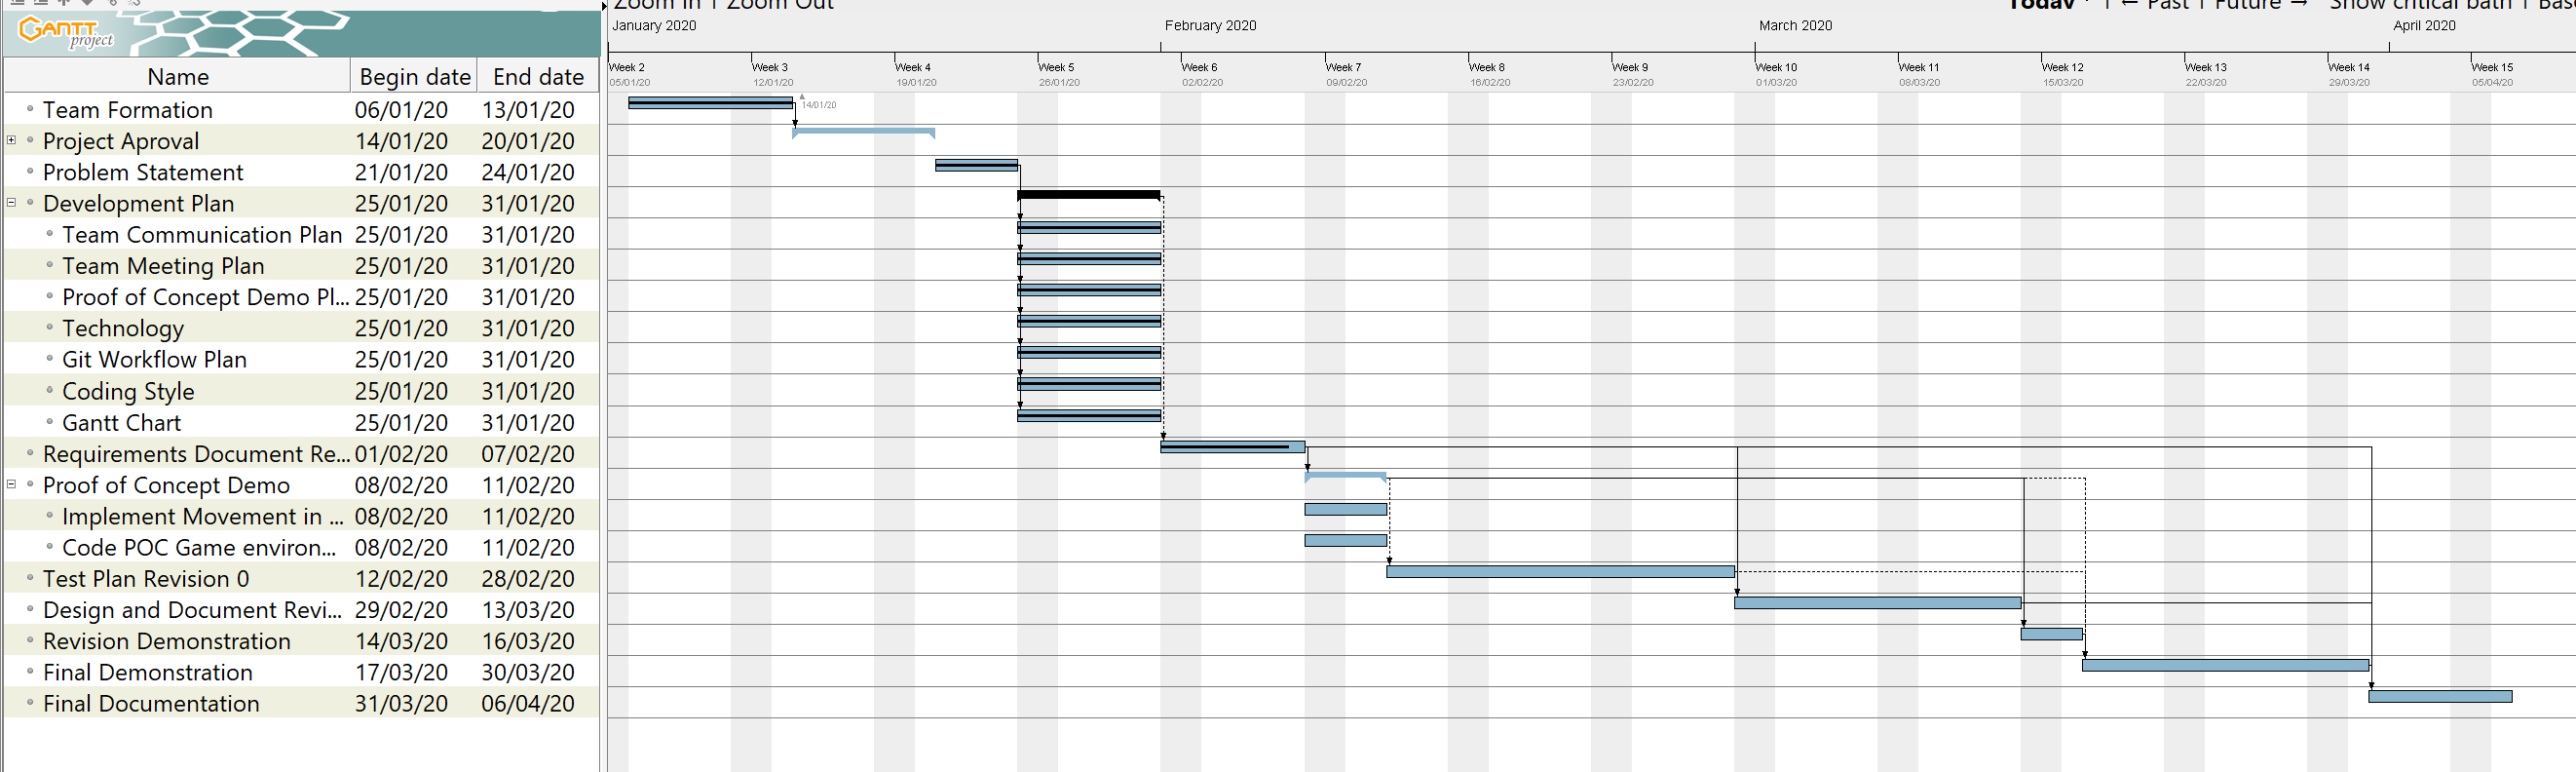
\includegraphics[width=\textwidth]{GanttChartSnapshotFeb9.png}
    \caption{Gantt Chart reflecting Proof of Concept updates}
    \label{fig:ganttchart}
\end{figure}

{\it This Gantt chart is updated throughout the project}

\subsection{Migration to the New Product}
\subsubsection{Requirements for Migration to the New Product}
N/A

\subsubsection{Data That has to Be Modified or Translated for the New System}
N/A

\subsection{Risks}
\subsubsection{Excessive Schedule Pressure}
There are serious time constraints on the project's development period. Therefore, the team be keen to stay on schedule or risk falling behind which would result in the final deliverable not functioning.

Probability: \sout{0} \textcolor{red}{15} percent

\subsubsection{Low Quality}
If the team looses sight of the end goal and becomes focused on trying to create something in-essential to the project, the main functionality of the end result will be full of issues, such as game lag. This could render the game not playable. Thus, the team must complete the core functions before creating fancy aspects.

Probability: 10 percent

\subsection{Costs}
The entire project will consist of the free to use coding language python and its corresponding free to use library pygame. Therefore, there is no monetary cost to the design and development of the game.

\subsection{User Documentation and Training}
\subsubsection{User Documentation Requirements}
The team will create a game controls outline and add it to the game settings. If the team has time, the first game level might come with a run through tutorial to help first time players understand how to play.

If the game is distributed publicly, a Read-Me file will accompany the game with instructions on how to download and install.

\subsubsection{Training Requirements}
There will be no learning curve; the controls must be intuitive enough to understand without training.

\subsection{Waiting Room}
A story line that plays out as the user beats levels as well as support for mobile devices will not be released as part of this version.

\subsection{Ideas for Solutions}
\sout{N/A} \textcolor{red}{The game could also be rendered using a different game engine such as Unity or Cry Engine 3. The highscore could be saved to a server database which would create a ultimate highscore for users to aspire to.}

\bibliographystyle{plainnat}

\bibliography{SRS}

\newpage

\section{Appendix}

\subsection{Symbolic Parameters}

The definition of the requirements will likely call for SYMBOLIC\_CONSTANTS.
Their values are defined in this section for easy maintenance.

\begin{table}[H]
\caption{\bf Symbolic Parameter Table}
\begin{tabular}{|l|p{0.5\linewidth}|l|}
\hline
\multicolumn{1}{|l}{\bfseries Symbolic Parameter} & \multicolumn{1}{|l|}{\bfseries Description} & \multicolumn{1}{l|}{\bfseries Value}\\
\hline
\textcolor{red}{ARROW\_KEYS} & \textcolor{red}{Keyboard keys that move the selector on the menus.} & \textcolor{red}{Keyboard Arrow Keys} \\
\hline
\textcolor{red}{KEYBOARD\_LEFT} & \textcolor{red}{Keyboard key that moves the onscreen character sideways to the left.} & \textcolor{red}{Left Arrow} \\
\hline
\textcolor{red}{KEYBOARD\_RIGHT} & \textcolor{red}{Keyboard key that moves the onscreen character sideways to the right.} & \textcolor{red}{Right Arrow} \\
\hline
\textcolor{red}{KEYBOARD\_JUMP} & \textcolor{red}{Keyboard key that moves the onscreen character vertically upwards.} & \textcolor{red}{Up Arrow}\\
\hline
\textcolor{red}{KEYBOARD\_ESC} & \textcolor{red}{Keyboard key that pauses the game mid play.} & \textcolor{red}{Escape Key}\\
\hline
\textcolor{red}{TEST\_USERS} & \textcolor{red}{A group of $20$ users chosen by the development team for their unique background and help round of an age range from 10 to 25. These users will also have to self identity as familiar with the orginal game.} & \textcolor{red}{N/A}\\
\hline
\textcolor{red}{INITIAL\_NAV\_TIME} & \textcolor{red}{N/A} & \textcolor{red}{$1$ minute and $30$ seconds.}\\
\hline
\textcolor{red}{UNDERSTAND\_TIME} & \textcolor{red}{N/A} & \textcolor{red}{$30$ seconds}\\
\hline
\textcolor{red}{MOVEMENT\_TIME} & \textcolor{red}{N/A} & \textcolor{red}{$10$ seconds}\\
\hline
\textcolor{red}{FRAME\_SPEED} & \textcolor{red}{N/A} & \textcolor{red}{$60$ frames per second}\\
\hline
\textcolor{red}{LOAD\_TIME} & \textcolor{red}{N/A} & \textcolor{red}{$3$ seconds}\\
\hline
\textcolor{red}{TEST\_ENTITIES} & \textcolor{red}{N/A} & \textcolor{red}{$100$ entities}\\
\hline
\textcolor{red}{INPUT\_RESPONSE} & \textcolor{red}{N/A} & \textcolor{red}{$3$}\\
\hline
\textcolor{red}{HIGHSCORE\_CORRECT} & \textcolor{red}{N/A} & \textcolor{red}{$3$}\\
\hline
\textcolor{red}{RUN\_TIME} & \textcolor{red}{N/A} & \textcolor{red}{$1$ hour}\\
\hline
\textcolor{red}{CRASH\_ACCEPTABLE} & \textcolor{red}{N/A} & \textcolor{red}{$0$ crashes}\\
\hline
\textcolor{red}{ROBUST\_ENTITIES} & \textcolor{red}{N/A} & \textcolor{red}{$1000$ entities}\\
\hline
\textcolor{red}{TIME\_ADDING} & \textcolor{red}{N/A} & \textcolor{red}{$5$ minutes}\\
\hline
\end{tabular}
\end{table}

\end{document}
